\graphicspath{{content/2_design/figures/}}
\section{Current Sensor}{\label{design_currentSensor}}
\subsection{Configuration}

The non-inverting amplifier configuration will be used for the current sensor. The gain, noise and rise time requirements should be analyzed to determine whether
a first or second order filter should be used.

\subsection{Gain}

The gain of the amplifier should be determined such that, when the maximum current flows through the sense resistor, the maximum voltage is output.
The maximum current of the motor should therefore be measured. This can be done by connecting the motor to a power supply (through an ammeter), stalling the motor, and reading the output current.

With a supply voltage of 6.4 V connected, the motor for this project read 740 mA, however different configurations may read between 1 and 1.5 A depending on the supply voltage and motor.
The average free-running current, however, is around 200 mA, and therefore a value of $I_{max} = \SI{400}{mA}$ will therefore be chosen to allow for some headroom while still maintaining adequate
resolution.

Since a sense resistor of $\SI{10}{\milli\ohm}$ is to be used, the maximum voltage through this resistor will therefore be 4 mV. Although this voltage level is small, it is expected, given that the resistance value is so small.
It is also desirable, as it shows that the circuit is not "stealing" too much power from the motor itself. Since it is not required to measure the motor current when stalled, gain will be calculated
based on a $\SI{5}{V}$ maximum rail voltage. A gain of $\frac{\SI{3.3}{V}}{\SI{4}{mV}} = 825$ is therefore chosen.

\subsection{Filter}

The requirements specify that a 10 mV signal at 1 kHz should be attenuated to less than 250 mV, i.e. should only have a gain of 25 and not 500. This means that
that a 1 kHz signal should be attenuated by $20 \log (\frac{825}{25}) \approx \SI{30}{dB}$. The specifications also require that the rise time, $t_r < \SI{100}{ms}$.
For a first order filter, this attenuation occurs at $10 \log \left[1 + \left(\frac{\SI{1}{kHz}}{f_{c(max)}}\right)^2\right] = 26 \therefore f_{c(max)} = \SI{32}{Hz}$ [\ref{filter_formulae}].
Also, the minimum frequency that will satisfy the rise time requirements for a first order filter is calculated using $f_{c(min) = \frac{2.2}{2 \pi t_r}} = \SI{3.5}{Hz}$ [\ref{filter_formulae}].
This shows that a first-order filter is adequate. A cutoff of $f_c = \SI{10}{Hz}$ is therefore chosen as a compromise between the two specifications.

\pagebreak

\subsection{Design}
Since a \nth{1} order filter will be used, a simple resistor-capacitor combination will be placed before the positive terminal.
Also, high resistor values should be chosen to limit current to below 150 uA.
\begin{itemize}
  \item Assuming $i_n = 0$, choose $\frac{V_{out(max)}}{R_1 + R_f} << 150 uA \therefore R_1 + R_f >> \SI{33}{\kilo\ohm}$. Choose $R_f = \SI{100}{\kilo\ohm}$.
  \item Since gain $G = 1 + \frac{R_f}{R_1} = 825$, $R_1 \approx \SI{120}{\ohm}$.
  \item Choose $C_i = \SI{100}{nF} \therefore R_i = \frac{1}{2 \pi \cdot \SI{10}{Hz} \cdot \SI{100}{nF}} = \SI{160}{\kilo\ohm}$. Choose $R_i = \SI{150}{\kilo\ohm}$ for $f_c \approx \SI{11}{Hz}$.
\end{itemize}

\subsection{Circuit Diagram}
The following figure details the final circuit design for the sensor and amplifier system.

\begin{figure}[h!]
  \centering
  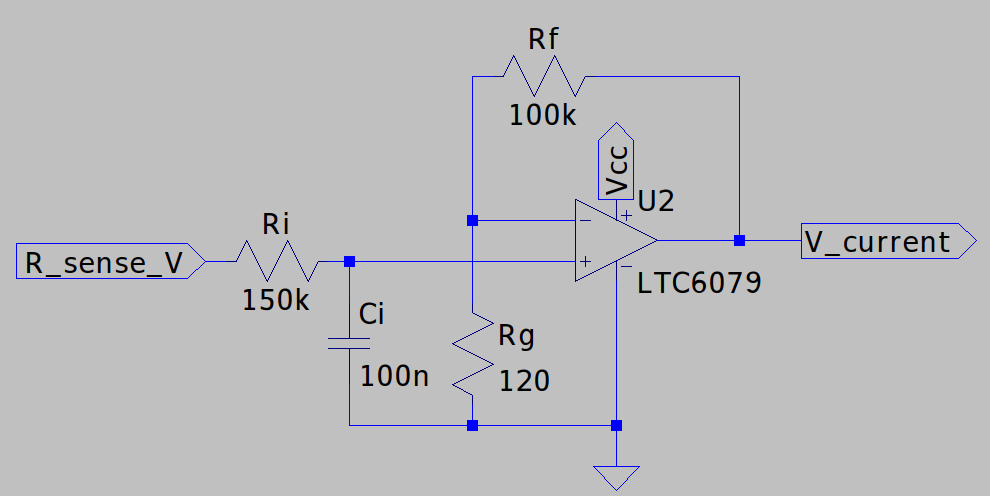
\includegraphics[width=.8\linewidth]{currentSensor_sim_circuit}
  \captionof{figure}{Current Sensor Circuit Diagram}
  \label{fig:circuit-diagram}
\end{figure}

A 3.3 V supply will be used to limit the voltage into the ESP, which will be reading the current sensor output.
Although there are benefits to a dual rail supply, that would prove impractical in the context of the larger system.

\pagebreak
